\documentclass[10pt, conference, compsocconf]{IEEEtran}

\newif\ifnoTBD \noTBDfalse

% Uncomment to remove TBD macros
%\noTBDtrue

%\ifx\pdftexversion\undefined
%  \usepackage[dvips]{graphicx}
%\else
%  \usepackage[pdftex]{graphicx}
%  \usepackage{epstopdf}
%\fi

\ifnoTBD
\def\TBD#1{\typeout{TBD not done: #1}}
\else
\def\TBD#1{\textcolor{blue}{TBD: #1}}
\AtEndDocument{\typeout{ *** ATTENTION: compilation is in DRAFT
    mode. There might still be TBD that appear in the document ***}}
\fi

\usepackage[usenames]{color}
\usepackage{xspace}
\usepackage{listings}
%\usepackage{type1cm}
\usepackage{eso-pic}
\usepackage{subfigure}
\usepackage{multirow}
\usepackage{url}
\usepackage{latexsym}
%\usepackage{hyperref}
\usepackage{comment}
\usepackage{graphicx}

%\hypersetup{%
%  pdftitle={},
%  pdfauthor={George Bosilca},
%  pdfkeywords={network scheduling}
%  bookmarksnumbered, pdfstartview={FitH},
%  linkbordercolor={0 0 0},
%  citebordercolor={0 0 0},
%  urlbordercolor={0 0 0},
%  pdfborder={0 0 0},colorlinks={true},
%  linkcolor={0 0 0},
%  urlcolor=none,
%  citecolor=white
%}%

%\setlength{\oddsidemargin}{0in}   % origin is (1",1") from top-left corner
%\setlength{\evensidemargin}{0.0in}
%\setlength{\textwidth}{6.5in}
%\setlength{\textheight}{9in}
%\setlength{\topmargin}{0.0in}
%\setlength{\headheight}{0pt}
%\setlength{\headsep}{0pt}

\newcommand{\ompi}{Open\,MPI\xspace}
\newcommand{\ftla}{FT-LA\xspace}
\newcommand{\scalapack}{ScaLAPACK\xspace}
\newcommand{\abft}{Algorithmic Based Fault Tolerance\xspace}

\usepackage{algorithmic}
\usepackage{algorithm}
\usepackage{color}
\usepackage{amsthm}
\usepackage{amsfonts} 
\usepackage{amssymb,amsmath} 
\usepackage{graphicx}

\begin{document}

\title{Enabling Application Resilience With and Without the MPI Standard}
\author{
  \IEEEauthorblockN{Wesley Bland}
  \IEEEauthorblockA{Innovative Computing Laboratory, University of Tennessee, Knoxville\\
					wbland@eecs.utk.edu}\\
}

\maketitle

\begin{abstract}

As recent research has demonstrated, it is becoming a necessity for large scale
applications to have the ability to tolerate process failure during an
execution. As the number of processes increases, checkpoint/restart fault
tolerance approaches requiring large concurrent state checkpointing become untenable and radically new
methods to address fault tolerance are needed. This work addresses these
challenges by proposing a novel approach to a minimalistic fault discovery and
management model.  Such a model allows application to run to
completion despite fail-stop failures. As a proof of concept, in addition to the
proposed fault tolerance model, an implementation in the context of the \ompi
library is provided, evaluated and analyzed.
% as well as providing a corresponding implementation in the context of the
% \ompi project.  allow applications to discover and tolerate failures while
% continuing execution, all while minimizing application involvement. It
% includes modifications to the \ompi runtime as well as MPI library to give the
% user options when deciding how best to implement fault tolerance.

\end{abstract}


\begin{IEEEkeywords}
Fault Tolerance, Message Passing Interface, Distributed Runtime
\end{IEEEkeywords}

\section{Introduction}

The insatiable processing power needs of domain science has pushed High
Performance Computing (HPC) systems to feature a significant
performance increase over the years, even outpacing "Moore's law"
expectations. Leading HPC systems, whose architectural history is listed
in the Top500~\footnote{www.top500.org} ranking, illustrate how massive
parallelism has been embraced in the recent years, leading to ever
growing systems featuring an impressive number of computing units;
current number 1, the K-computer has half a million cores, and even with
the advent of GPU accelerators, it requires no less than 73,000
cores for the Tsubame 2.0 system (\#5) to breach the Petaflop
barrier. Indeed, the International Exascale Software Project, a group
created to evaluate the challenges on the path toward Exaflop class
machines, has published a public report outlining that a massive
increase in scale will be necessary, when considering probable advances
in chip technology, memory and interconnect speeds, as well as
limitations in power consumption and thermal envelope~\cite{iesp}.
According to these projections, as soon as 2014, billion way parallel
machines, encompassing not only millions of cores, but also tens of
thousands of nodes, will be necessary to achieve the desired level of
performance. Even considering extremely optimistic advances in hardware
reliability, probabilistic amplification entails that failures will be
unavoidable, becoming common events. Hence, fault tolerance is paramount
to maintain scientific productivity.

Already, for Petaflop scale systems the issue has become pivotal. On
one hand, the capacity type of workload, composed of a large amount of
medium to small scale jobs, which often represent the bulk of the
activity on many HPC systems, has traditionally been left unprotected
from failures, resulting in diminished throughput due to failures. On
the other hand, selected capability applications whose significance is
motivating the construction of supercomputing systems are protected
against failures by ad-hoc, application-specific approaches, at the
cost of straining engineering efforts, translating in high software
development expenditures. Two long lasting issues have hindered
ubiquitous adoption of streamlined fault tolerance techniques: first,
the traditional checkpoint based approaches incur a steep overhead on
failure-free operations; second, the dominant approach for programming
parallel distributed memory systems, the MPI standard~\cite{MPI22} and
its implementations, offer extremely limited support for software
fault tolerance approaches, which effectively limit the spectrum of
options available to applications to periodic checkpointing and
rollback recovery.

Several propositions have emerged from the ongoing MPI-3
forum\footnote{\url{http://meetings.mpi-forum.org/mpi3.0\_ft.php}},
toward improving the expressivity of MPI with regard of fault tolerant
techniques. However, it is yet unclear as to wether these propositions
will prove successful enough to be blessed by the forum as they still
incur synchronization overhead on failure-free scenarios. The current
MPI-2 standard leaves open an optional behavior to qualify as a "high
quality implementation", regarding failures: according to this
specification in the case of an MPI\_ERRORS\_RETURN error handler,
when the MPI library detects a failure it should return control to the
caller. This is at the opposite of the default mass-suicide action
that all notable MPI implementations undergo in case of a failure. In
this paper, we investigate the modifications that are required, inside
the MPI implementation, to enable this behavior strictly within the
scope of the current standard. We then describe how algorithm-based
recovery techniques, illustrated by the most useful QR factorization,
are able to leverage this behavior, to perform an inexpensive recovery
that completely avoids costly periodic checkpointing, and rollback
recovery. Although the proposed technique uses checkpointing to save
the state of the application, it does so only after the system was
affected by a failure, and the recovery operation could be qualified as forward
recovery, since it does not make the application rollback.

The remainder of this paper is organized as follows. The next section
presents typical fault tolerant approaches and related works to discuss
their requirements and limitations. Then, we present in
Section~\ref{sect:ompi} the On-Demand Checkpointing approach, and the
minimal support required from the MPI implementation. 
Section~\ref{sec:ftla} presents the use case: a fault tolerant
version of the QR algorithm, and how it has been modified to fit the
proposed paradigm. Section~\ref{sec:model} presents a performance model to
assess the efficiency of both periodic checkpointing with rollback
recovery and On-Demand Checkpointing, and
Section~\ref{sec:experiments} presents an experimental evaluation of
the implementation.
%Section~\ref{sec:ompi} investigates
%the intricacies of the MPI runtime



%\section{Background \& Related Work}
\label{sect:background}

% Discuss some MPI-3 related proposals and issues

%Among the issues
%raised during the readings of the proposals, were the fact that these
%approaches will still incur a significant overhead on failure free
%operations, by requiring periodic \emph{consensus}

\subsection*{Background}

Message passing is the dominant form of communication used in parallel
applications, and MPI is the most popular library used to implement
it. However, as fault tolerance becomes a growing concern for
application developers, users have encountered some challenges with
the current MPI Standard that limit their options of fault tolerance
methods. The primary form of fault tolerance today is to periodically
write a checkpoint to disk.  While this method is effective in
allowing applications to recover from failures by restarting the work
from a previously saved point, it causes serious concerns on the
scalability~\cite{ExaScaleResilience09}. Moreover, such proactive
approach to fault tolerance requires a good idea of how many faults
might hurt the system, with which frequency and on what nodes. Many
works have discussed the optimal checkpointing period in the hope that
as few as possible of these preventive actions are taken by the
application~\cite{Young:1974, Gelenbe:1979, Plank01, Daly:2006,
  PreventiveCheckpointing11}. Unlike these works, the work presented
here focuses on {\it forward recovery}: checkpoint actions are taken
only {\emph after} a failure is detected, make it unnecessary to
hypothesize on an optimal checkpoint interval. The checkpoint interval
is optimal, by definition, as there will be one checkpoint interval by
effective fault.

An alternative approach to rollback recovery is to take advantage of
the properties of the application to design it as naturally fault-tolerant. This
technique is traditionally called \abft \cite{huang1984algorithm}. The
algorithm itself includes modifications, or additional steps, to cope
with the loss of some of its data. It includes a modification of the
algorithm, usually to maintain redundant information in the data
during the life of the application, and a recovery procedure that
works only with the data remaining after the failure is detected, and
reconstructs the missing data using additional computation and
communication. To support such an algorithm, the underlying
programming environment must however provide a way to communicate
after the failure occurs on one of the processes.

The current MPI Standard (MPI-2.2,~\cite{MPI22}) does not provide
significant help to deal with that type of behavior. Section~2.8
states in the first paragraph: ``\emph{MPI does not provide mechanisms
  for dealing with failures in the communication system. [...]
  Whenever possible, such failures will be reflected as errors in the
  relevant communication call. Similarly, MPI itself provides no
  mechanisms for handling processor failures.}'' Failures, be they due
to a broken link or a dead process are considered as resource
errors. Later, in the same section: ``\emph{This document does not
  specify the state of a computation after an erroneous MPI call has
  occurred. The desired behavior is that a relevant error code be
  returned, and the effect of the error be localized to the greatest
  possible extent.}'' So, for the current standard, process or
communication failures are to be handled as errors, and the behavior
of the MPI application after an error has been returned is left
unspecified by the standard. However, the standard does not prevent
implementations to go beyond its requirements, and on the contrary,
encourages high-quality implementations \emph{to return} errors once a
failure is detected.

Unfortunately, most of the implementations of the MPI Standard have
taken the path of considering process failures as unrecoverable
errors, and the processes of the application are most often killed by
the runtime system, when a failure hits any of them. The runtime
system then returns with an error code, signaling the failure of the
run, leaving no other choice to the user but to run a new parallel
execution.

The MPI forum is currently examining options for the future direction
of MPI for MPI-3. One of the workgroups is dedicated to propose a
standard form of MPI-supported fault tolerance. The proposal outlines
a method of run-through stabilization which allows the application to
acknowledge and repair communications, both collectively and between
specific ranks in a point-to-point way~\cite{Hursey11MPI3FT}. The
emphasis of the proposal is a set of "validation" functions which the
application is required to call to repair and re-enable communication within
an MPI communicator containing a failed process. To repair point to
point wildcard receives, the application needs to collectively call the function
MPI\_COMM\_REENABLE\_ANY\_SOURCE. To repair collective communication
within a communicator, the application needs to call the function
MPI\_COMM\_VALIDATE.  These functions give the MPI implementation an
opportunity to acknowledge failures and discover or ensure that other
MPI processes also acknowledge the same failures. It also gives the
MPI library a chance to repair communication channels between
remaining processes, optimizing communication topologies if possible
and necessary.

While this method of fault tolerance is sufficient for \abft, it is
not without its drawbacks. The calls necessary to recover from
collectives incur a non-trivial overhead even during the fault free
case. MPI\_COMM\_VALIDATE requires a distributed consensus algorithm
which is currently best implemented at log
scale~\cite{Hursey11LogConsensus}. While this level of overhead is
better than the current state of the art of periodic checkpointing, it
still presents a significant cost that not all applications want or
need to pay to check the validity of the communicators. Most
importantly, this proposal does not yet include process recovery,
which is left to a future proposal to the MPI forum.

% Discuss issues in general with FT-MPI like approaches, besides the 
% sheer problem of standard adoption

% Explain why it is not believed that ABFT can perform without REPLACE 
% or BLANK, or leave it for next section ?

\subsection*{Related Work}

FT-MPI~\cite{fagg2000ft} is an MPI-1 implementation which added
extensions to the MPI standard to give users options for their
\abft. FT-MPI proposed to change the MPI semantics of some of the
calls, to enable continuing the execution of the parallel application
after a failure hits the system, and to rebuild the communicators, thus
re-enabling communications. This approach has been proven successful,
and some applications have been implemented relying on the features of
FT-MPI. However, these modifications of the standard were not imported
in the official MPI standard, and no other MPI implementation took the
same approach. The lack of large distribution of the FT-MPI
implementation prevented a large base of users from implementing their
solution based on this proposition.

%  One of
% the solutions implemented in FT-MPI was to introduce a new MPI\_Errhandler
% called MPI\_ERRORS\_BLANK. This MPI\_Errhandler replaced the position of the
% failed processes inside a communicator with MPI\_PROC\_NULL. By using this
% semantic, the remaining MPI calls could function normally as communication with
% MPI\_PROC\_NULL always succeeds. When FT-MPI encountered a fault, it destroyed
% all MPI Communicators and required that the application recreate them to account
% for the failed processes. While this was a useful step in allowing the most
% level of flexibility from the application's perspective, it made recovery very
% complex and added a large overhead.

% FT-MPI is another form of fault tolerance that can be successful for some, but in
% applications that require that all processes be running to reach successful
% completion, having a hole in the communicator is not a valid solution. The
% failed processes need to somehow be recovered.

%\TBD{Anything needed from the QR side of things?}

Besides the works that have been cited previously to present the
problem statement, the different approaches that have been proposed,
and how this approach is original, the article by W. Gropp and E. Lusk
in 2004 \cite{Gropp:2004:FTM:1080704.1080714} is the work closest to
the On-Demand Checkpointing, from the MPI requirement perspective.  In
this article, the authors explain how the standard can be interpreted,
or slightly modified, to allow for a form of fault tolerance. They
consider different approaches: periodical checkpointing; using
inter-communicators and separate MPI applications to contain an error
in an MPI application; modifying the MPI semantics; or propose new
extensions. However, the last three propositions demand more from the
MPI implementation than we require in this work: for example, the MPI
library is supposed to continue its normal execution, if the error was
located in another MPI application, connected with the one subject to
the error through an inter-communicator. In our work we do not even
require such a step: the only
demand on the MPI implementation is that it does not forcibly kill the
living processes without letting them take a checkpoint, but returns
an error. Once this is ensured, no requirement from any MPI call is
needed.

Moreover, we illustrate the well soundness of our approach using a
non-trivial algorithm: a QR factorization, that is made fault tolerant
using the modified \ompi, and the On-Demand Checkpointing
technique. We demonstrate that this approach is functional, and
evaluate its performance at large scale.

\section{Related Work}\label{sect:related}

% Why coordinated checkpointing is no longer scalable

The current industry standard for failure handling is rollback recovery with
periodic checkpoints to disk, and many libraries have been implemented to
support this behavior~\cite{Duell:tr, Litzkow:1997wd, Plank:1994wz,
Zhong:2001tq}. This has been an effective recovery model for many years and
continues to be an area of research to prolong its
usefulness~\cite{BautistaGomez:2011hg, BuntinasFGCS2008, Elnozahy:2002p3769},
despite the increase in fault frequency and the hierarchization of the
underlying hardware architecture.  However as machines continue to scale,
concerns have been raised about the scalability of rollback
recovery~\cite{Cappello:2009hs}.  The time spent performing recovery operations
is expected to exceed the MTBF in the next generation of supercomputers, causing
any large-scale applications to enter a cycle of recovery where no useful
computation occurs.

% Resilience workshop report

In February 2012, the Department of Defense and Department of Energy conducted
research~\cite{Daly:2012vg} to outline the necessity for resilience at extreme
scale, specifically for exascale computing. They affirmed the likelihood that
exascale systems will have a shorter MTBF than existing systems. They also
recommended that ``a `light-weight' approach, i.e., effective and easy to
implement, is preferable to a `full-featured' alternative.'' By attempting fewer
features, each library can focus on creating a scalable and efficient
implementation while promoting simplicity and reducing unnecessary features. The
agencies also discussed possible redundancy approaches (discussed
in~\cite{BosilcaINRIARep7950, Ferreira:2011fb}), describing them as ``not
practical because they require 2-3x more energy''. The price of redundancy must
not only include the obvious loss of computing time from executing duplicate
codes across multiple processors, but also the up-front costs of purchasing
extra hardware on which to execute the redundancy.

% Describe ABFT

Out of these problems have arisen a new class of algorithms that allow different
methods of resilience. These algorithms support what is called Algorithm Based
Fault Tolerance (ABFT). They have been designed to support a recovery model that
does not require all processes to participate in the recovery simultaneously or,
perhaps, ever at all. Huang and Abraham first explored these
algorithms~\cite{Huang:1984kt} for soft errors in systolic arrays, but research
has expanded to create ABFT techniques for many algorithms~\cite{Du:2012je, Plank:1995hv}.

% RTS Proposal

To support these new algorithms, applications require support from their
libraries. One of the most popular communication libraries used by large scale
applications is the Message Passing Interface (MPI), the contents of which are
determined by the MPI Forum. The MPI Forum has previously considered proposals
to add fault tolerance capabilities to the MPI Standard. In 2011, a proposal was
brought forth~\cite{Hursey2011RTS} titled ``Run-Through Stabilization'' which
discussed a wide range of fault tolerance capabilities to provide for users by
defining the behavior of MPI following a process failure as well as introducing
new constructs to provide strong consensus between processes. The MPI Forum
decided to reject the proposal, but the work led to more research in the field
of resilience in MPI, including the work being proposed in
Section~\ref{sect:ulfm}.

% FT-MPI

Outside of the MPI Forum, work has been done to provide fault tolerance to MPI
applications. FT-MPI~\cite{FaggFTMPI} was an MPI-1 compliant implementation of
the MPI Standard which added new capabilities for fault tolerance. It included
automatic recovery models for failures including: shrinking MPI communicators to
automatically remove failed processes, leaving holes in the communicators while
allowing communication to continue, and destroying and rebuilding the
communicators to retain communication patterns and groups. FT-MPI was never
adopted into the MPI Standard but continued as a research project for many
years. 

\section{Runtime} \label{sect:runtime}

This section summarizes the modifications that were necessary for us to create our resilient runtime layer. Details of our implementation of the work outlined in this section can be found in~\cite{Bland:CCGrid12}. The major requirements fall into three categories: failure detection, failure notification, and failure handling.

\subsection{Failure Detection} \label{subsect:failure_detection}

While failure detection can take place throughout an applications layers, the runtime layer is the most well positioned to discover failure quickly. Because it manages process launching and communication channels, it can quickly detect failures. Once it detects a failure, it can begin the process of failure notification. 

\subsection{Failure Notification} \label{subsect:failure_notification}

When a failure is detected, the runtime environment is responsible for propagating knowledge of the failure to all appropriate parts of the application. This includes the runtime environments on other nodes, as well as to the MPI layer of the application.

\subsection{Failure Handling} \label{subsect:failure_handling}

Concurrently with failure notification, the runtime must also perform failure handling tasks to stabilize the runtime environment and allow the application to continue. This includes route healing, where communication channels within the runtime environment must adapt to losing a node as a potential routing hop. It also includes ensuring message consistency to prevent repeated failure notification and to prevent loss of messages as much as possible.
\section{MPI} \label{sect:mpi}

% What does the current standard do?

The current MPI standard does not provide much guidance for applications in
presence of faults. According to the standard, when implementing a high-quality
MPI library, the application should regain control following a process failure.
This control gives the application the opportunity to save its state and exit
gracefully, rather than the usual behavior of being aborted by the MPI
implementation itself. This makes continuing meaningful execution very difficult
and usually requires the application to restart itself from a previously saved checkpoint.

% What kind of FT can we do with it?

% One opportunity to use the current MPI standard without modification is to use
% the MPI error handler MPI\_ERRORS\_RETURN rather than MPI\_ERRORS\_ABORT. This
% would allow the application to write a checkpoint which it can use to restart
% itself from the current point with a clean MPI library. However, this requires
% an application that is already fault tolerant and can continue without the failed
% process or can recreate the lost data from the failed process. While this class
% of Application Based Fault Tolerant algorithms does exist, it does not encompass
% the vast majority of applications.

% What departures did we create from the standard?

Our work deviates from the current standard to provide a more flexible suite
of tools to implement fault tolerance. 
%
If a process failed during an MPI call, the call will return an error code to
reflect the failure. This allows the application to know that a process has
failed and to perform any internal recovery operations necessary. Once the
application has been alerted via the MPI return code, the application will not
receive another notification until a new process fails. By not requiring an
acknowledgment from the remaining processes, our method of fault tolerance
imposes as little burden on the applications as possible and allows failure free
executions to incur the minimum amount of overhead.

As most of the MPI applications take advantage, in addition from point-to-point
message, of collective communications, we took a particular interest in
providing a clear semantic of how fault can integrate with collective
communications. We are implementing fault
tolerant collective operations which allow the application to run collectives
over MPI\_Communicators including failed processes. For collectives which do not
include any data, such as MPI\_Barrier, this is simple enough operation.  For
collectives which require data combination, such as MPI\_Gather or MPI\_Reduce,
this can be a slightly more complicated task. However, all of the MPI collective
operations can eventually be simplified to a communicator pattern with some
amount of data, which may or may not be combined with or without an operation in
the process. When determining how many processes to include in the collective
operation, our MPI library does not include the failed processes. Also, when a
process fails during a collective, the operation is updated to remove the failed
process. Once the participating group is determined, we can continue the MPI
collective as if no failures occurred.

This work will also eventually include process recovery which will allow the
application to decide to recreate the failed process by launching a new MPI rank
on a fault free node. The user will be responsible for bringing the new rank
back to the point of the failure, but this will support another set of
applications which require a specific number of processes to continue in the
presence of a process failure.  The specifics of the process recovery techniques
are not yet ready for publication.

\section{Performance Discussion} \label{sect:experimental}

\begin{figure*}[t]
  \centering
  \subfigure[\small One Process failing at a time]{
    \label{fig:onebyone}
    \includegraphics[scale=0.65]{figures/even.pdf}
  }
  \subfigure[\small Two concurrently failing processes]{
    \label{fig:burst}
    \includegraphics[scale=0.65]{figures/burst.pdf}
  }
  \caption{Token Roundtrip Time with Evenly Failing Processes}
  \label{fig:even}
\end{figure*}

%\begin{figure*}[t]
%  \centering
%  \subfigure[\small N/2 Processes Failing at Midpoint]{
%    \label{fig:major}
%    \includegraphics[scale=0.50]{major.pdf}
%  }
%  \subfigure[\small N-2 Processes Failing at Midpoint]{
%    \label{fig:critical}
%    \includegraphics[scale=0.50]{critical.pdf}
%  }
%  \caption{Token Roundtrip Time with Many Simultaneous Failing Processes}
%  \label{fig:many}
%\end{figure*}

\begin{figure*}[t]
  \centering
  \subfigure[\small Detection Time for Failures]{
    \label{fig:detection}
    \includegraphics[scale=0.65]{figures/epochs-lines.pdf}
  }
  \subfigure[\small Overhead Introduced by Changes]{
    \label{fig:overhead}
    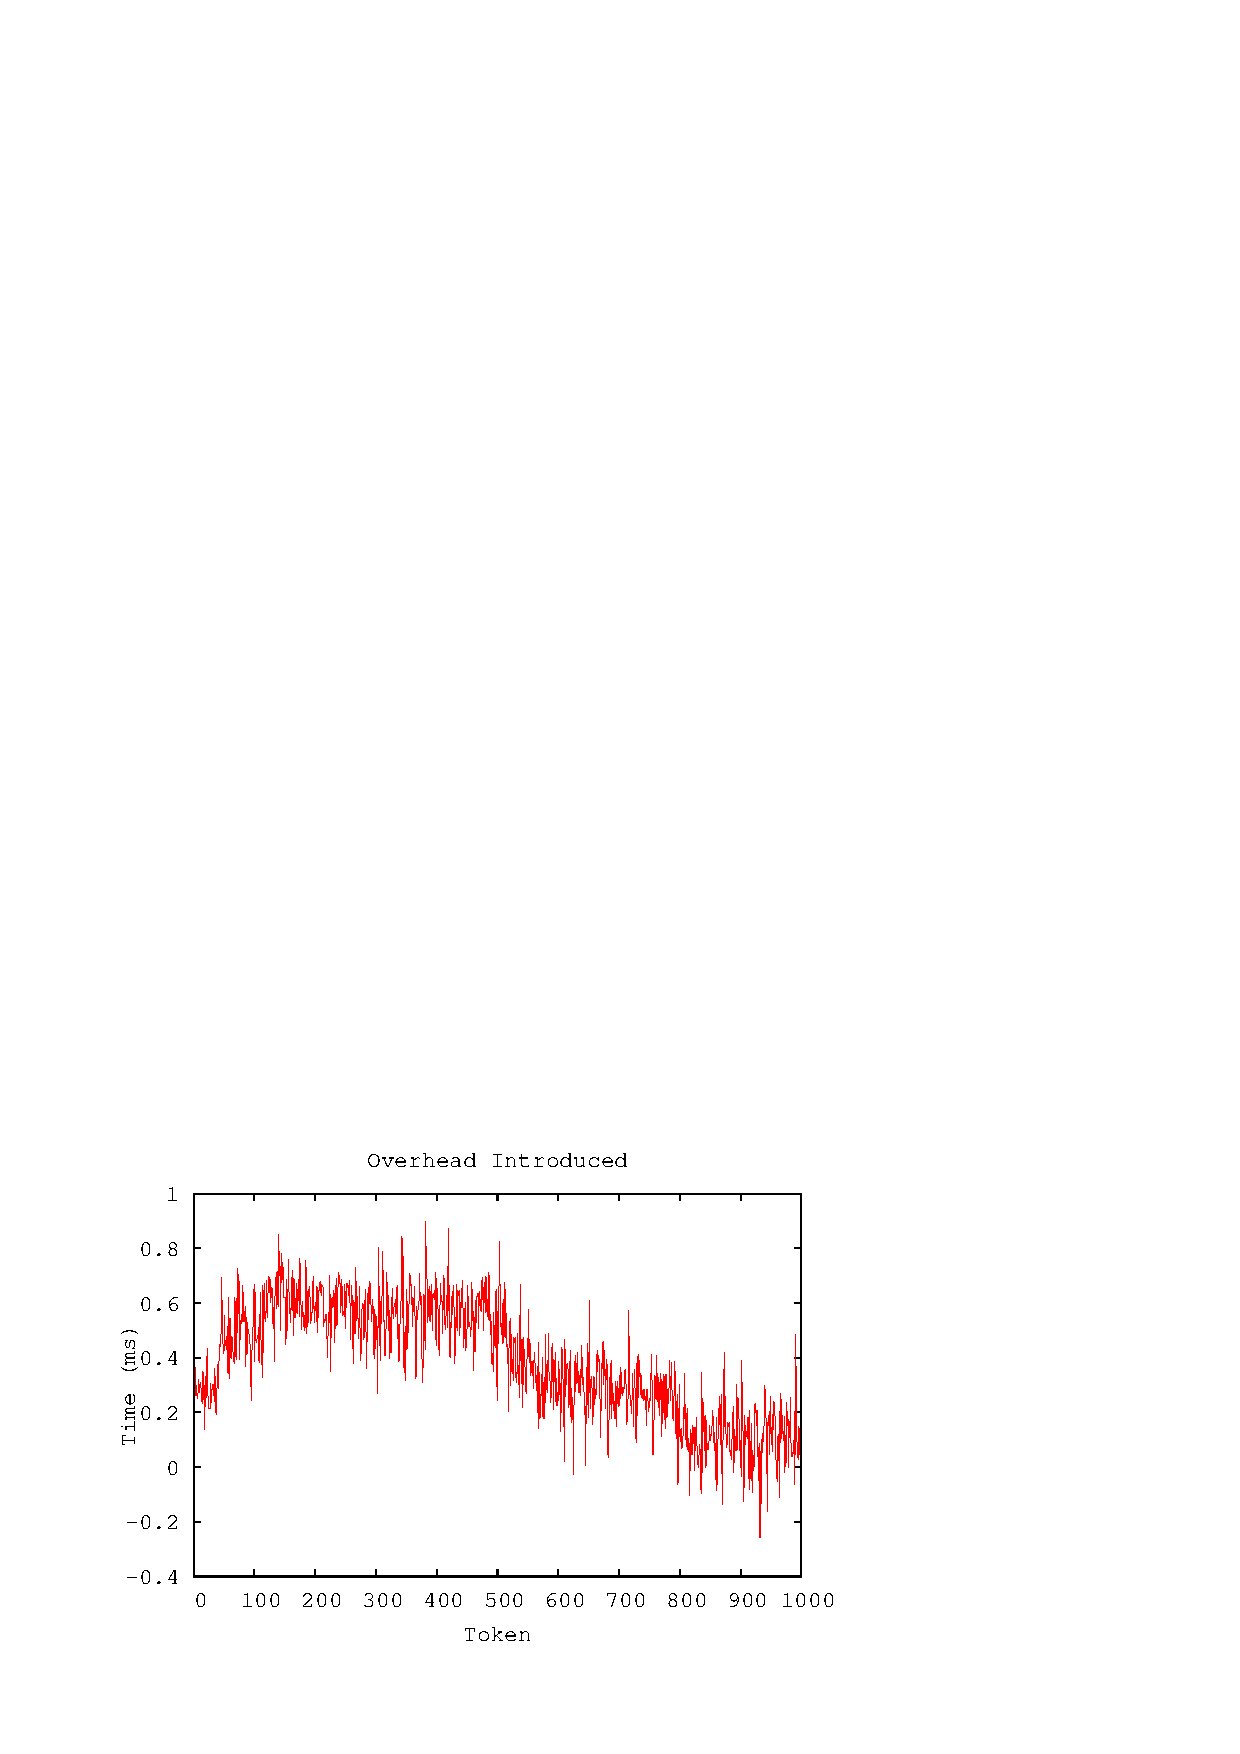
\includegraphics[scale=0.65]{figures/overhead.pdf}
  }
  \caption{Overheads of the Resilient Runtime}
  \label{fig:overheads}
\end{figure*}

% -- Runtime --
In this section we describe the results of our work to this point. First we present a model
to describe the expected results of our resilient runtime's failure notification
method. Second, we will demonstrate the observed values derived from our tests
performed on a 64 node cluster within Grid5000. \footnote{Experiments presented
in this paper were carried out using the Grid'5000 experimental testbed, being
developed under the INRIA ALADDIN development action with support from CNRS,
RENATER and several Universities as well as other funding bodies (see
https://www.grid5000.fr)}

\subsection{Performance Model} \label{subsect:performance_model}
% Describe the model that our runtime is expected to fit within.

We devised a model of the expected failure detection behavior of our runtime
system. Let $T$ be the initial routing topology of the system. Let $L_T(d, f,
H)$ be the time it takes process $d$ to notice a failure of process $f$, knowing
that $\forall q\in H$, $q$ is also failed (potentially before $f$). We call
$L_T(d, f, H)$ the latency of detection of $d$ for $f$ knowing $H$.

$$L_T(d, f, H) \leq \alpha_0 + \gamma D_{T \backslash H \cup \{f\}}(f, d)$$

Where $\alpha_0$ is the time taken by an immediate neighbor of $f$ to detect its
failure, $\gamma$ is the point-to-point message latency, and $D_{T \backslash H
\cup \{f\}}(f, d)$ is the distance (in number of hops) between $f$ and $d$ in
the routing topology, $T \backslash H\bigcup \{f\}$. Note that this distance
could shrink as processes between $f$ and $d$ in the routing topology fail.

Whatever the history of failures $H$, if $|T| = n$, then $D_{T \backslash H}(s,
d) \leq \log_2(n)$. This is true because the routing layer we use is a binomial
tree, which has a maximum depth of $log_2(n)$. Also, when repairing the routing
tree after a failure, the routing layer does not add new hops, it only mends the
routes by removing failed processes from the topology and creating links between
the next surviving neighbors both above and below $f$. Thus, for system $Bin(n)$
with $n$ processes initially, with a fault tolerant binomial tree routing layer,

$$\forall d, f\in Bin(n), \forall H \subseteq Bin(n),$$
$$L_{Bin(n)}(d, f, H) \leq \alpha_0 + \gamma \log_2(n)$$

This shows that our improved routing topology should perform no worse than a
fault free one following a process failure.

\subsection{Performance Data} \label{subsect:performance_data}

% Ring test with binomial routing
% Emphasize "Proof of Concept" rather than large scale performance runs

When validating the runtime work described in Section~\ref{sect:runtime}, our
goal was to devise a test that would confirm its correctness while being simple
to describe and understand. It should be emphasized that this is not necessarily
representative of a specific application, but it does demonstrate that the
improved runtime would be able to support a full application in the presence of
a process failure. It is designed to show that the runtime can heal its routing
layers following multiple and catastrophic process failures. Once a resilient
MPI layer is built on top of the runtime, a full application could be tested
with MPI semantics.

Our test is a ring test which dispatches multiple tokens from process 0. These
tokens are passed around the ring in increasing sequential order until they
reach process 0 again where various measurements are made. This is a simplistic
test and therefore not designed to demonstrate the recovery of a lost token,
however the test could easily be modified to demonstrate that behavior as
described by Hursey~\cite{Hursey:vb}. Process 0 generates 4000 tokens and passes
them along. As the tokens are passed around the ring, the test generates
failures at predetermined times to give an idea of the behavior of the runtime
with different failure patterns. The loss of tokens gives an idea of how long
the routing layer took to patch itself and continue sending tokens to the next
living process.

% Describe the graphs

Figure~\ref{fig:even} shows the round trip time of each of the tokens as the
failures are generated within the system. Each graph shows both the time from a
failure free run and a run with a specific failure pattern. The graphs also
show how many hops each token traversed while traveling around.

% Compare ring/token test FF vs. failure

In Figure~\ref{fig:onebyone}, processes fail one at a time in evenly spaced
intervals until only 2 processes remain. As each process fails, the round trip
time decreases linearly. This is the expected behavior as each token must
traverse fewer processes until it reaches process 0 again. The number of hops
decreases slowly as each process fails, but the round trip time with failures
actually decreases at a greater rate temporarily. This is because the buffers at
the first few processes become full at the beginning of the run when the tokens
are still being generated. As the buffers clear the first few processes, the
round trip time stabilizes.% into a linear speedup.

In Figure~\ref{fig:burst}, processes fail in groups of two. This shows that the
runtime can withstand larger groups of processes failing at roughly the same
time.
% This would simulate a two processor node failing at once.
 The gaps in the
graph show the points at which some tokens are lost. This is expected as the
application makes no attempt to recover or regenerate tokens temporarily hosted
by failed processes, and simply continues to run with whatever tokens return
back to the originating process.

%% Kill 1/2 in middle
%Figure~\ref{fig:major} introduces much larger failures at a time. In this test,
%half of the processes fail all at once at the midpoint of the run. While it
%takes the runtime some time to discover all of the failures, as illustrated by
%the larger number of lost tokens, it does eventually recover from the losses and
%any tokens that were not on one of the failed processes at the time of the
%failure continue around the ring until process 0 receives them again.
%
%% Kill p - 2 in middle
%Figure~\ref{fig:critical} introduces a critical failure. In this test, all but
%two processes are killed at the same time at the midpoint of the run. Again, the
%runtime requires a discovery period before stabilizing, but it is able to
%recover and continue delivering the remaining tokens back to process 0.
%Figures~\ref{fig:major} and~\ref{fig:critical} are encouraging as they show that
%the runtime can withstand any number of failures at any time. This
%implementation can withstand concurrent or consecutive failures without
%requiring any minimal ``cooling off'' period between failures.

Our runtime is also able to handle failure rates much higher than one or two
processes at a time. In other tests, we were able to handle rates of $n/2$ or
$n-2$ simultaneous failures. This is encouraging as it shows that the runtime
can withstand any number of failures at any time. The failures can occur
concurrently or consecutively without requiring a ``cooling off'' period between
failures.

% Detection Time
Figure~\ref{fig:detection} shows the detection and notification time for each
failure. It uses the same case as figure~\ref{fig:onebyone} where failures occur
evenly throughout the lifetime of the application. Each line represents the
detection time of each epoch among all the processes, collected using the ad-hoc
fault handler. 
% To reduce the effect of clock drift, the time is measured from
% the beginning of the local application rather than attempting to synchronize
% with a single value from process 0. 
When the line is straight, it
demonstrates that the latency of detection and notification is
relatively low among all the remaining process. This figure shows that the
detection time for the all processes is very tight, demonstrating that all
processes can maintain a consistent view of the current epoch. The earlier
epochs have a slightly varying detection time as the notification messages have
further to travel through the routing layer, but as the tree becomes smaller as
it is repaired, the oscillations decrease, demonstrating a much smaller window
of time for each epoch.

% Overhead
Figure~\ref{fig:overhead} shows the overhead that was introduced by modifying
the \ompi source code. It compares the runtime of a fault-free case using both
our implementation of the \ompi runtime, and the revision 24614 of the \ompi
trunk. The overhead was measured on a local 8 node development cluster with
minimal system noise to eliminate outside effects on the data. We subtract the
round trip time for each token in the resilient version of \ompi from the same
test using the trunk version of \ompi. The results show that the changes made to
the code actually had little impact on performance in the fault-free case.
Variations can be explained by the network jitter and the small increase in the
header size of the messages due to the epoch algorithm.


\section{Conclusion}
\label{sect:conclusion}

Many responsible voices agree that sharp increases in the volatility of future,
extreme scale computing platforms are likely to imperil our ability to use them
for advanced applications that deliver meaningful scientific results and
maximize research productivity. Since MPI is currently, and will likely continue
to be -- in the medium-term -- both the de-facto programming model for
distributed applications and the default execution model for large scale
platforms running at the bleeding edge, it is the place in the software
infrastructure where semantic and run-time support for application faults needs
to be provided.

The \ulfm proposal is a careful but important step forward toward accomplishing
this goal delivering support for a number of new and innovative resilience
techniques through simple, familiar API calls, but it is backward compatible
with previous versions of the MPI standard, so that non fault-tolerant
applications (legacy or otherwise) are supported without any changes to the
code. Perhaps most significantly, applications can use \ulfm-enabled MPI without
experiencing any degradation in their performance, as we demonstrate in this
paper. Some of these applications along with other portable libraries are
currently being refactored to take advantage of \ulfm semantics.

The author would like to acknowledge his co-authors in the full
paper~\cite{Bland:2012tp}: Aurelien Bouteiller, Thomas Herault, Joshua Hursey,
George Bosilca, and Jack J. Dongarra.


\newcommand{\BIBdecl}{\setlength{\itemsep}{0.03\baselineskip}} 
\bibliographystyle{IEEEtran}
\bibliography{resil-mpi-ccgrid}

\end{document}

